\section{Introduction}
The task of automatic charge prediction is to determine appropriate charges, 
such as \emph{fraud}, \emph{larceny} or \emph{homicide},  for a given case by analyzing its 
textual fact description.  Such techniques are crucial for legal assistant systems, where
users could find similar cases or possible penalties by describing a case with their own words,
% \orange{This kind of systems are helpful for people who have no legal background and know nothing about the legal jargon, since extra support from the legal professionals are usually expensive.}
even they have no legal background and 
know nothing about the legal jargon, \orange{since extra support from the legal professionals are usually expensive.}

%Determining appropriate charges, such as \emph{fraud}, \emph{larceny} or \emph{homicide}, 
%based on the fact description of a case is one of the key components in legal assistance systems.
% when the user would like to query the system by describing the case, and it is \orange{even more important} when the user has no idea of the legal basis of a case, where the only input he (or she) can give is the fact description of the case. 
% In this situation, predicting appropiate charges would help us to provide the user with relevant  
%For example, if the user wants to find similar cases, one can use the predicted charges of the query case to filter out irrelevant results. And if the user wants to know the possible penalties \orange{regarding a case}, one also need to decide appropriate charges first.



%In these situations, we need to predict appropirate charges based solely on the fact descriptions of a case. 
However, predicting appropriate charges based on fact descriptions is not trivial:
(1) The differences between two charges can be subtle, for example, in the context of criminal cases in China, 
distinguishing \emph{intentional homicide} from \emph{intentional injury} would require to determine, 
from the fact description, whether the defendant  \textit{intended to kill} the victim, 
or just \textit{intended to hurt the victim, who, unfortunately, died of his severe injury}.
%but in the cases where the victim is dead.
% distinguishing \emph{intentional homicide} from \emph{negligent homicide} would require detailed analysis of the behavior of the defendant.
% and \emph{acceptance of bribes} differs from \emph{acceptance of bribes by a non-state functionary} in the occupation of the defendant. 
(2) Multiple crimes may be involved in a single case, which means that we need to conduct charge prediction in the multi-label classification paradigm. 
(3) Although we can expect an off-the-shelf classification model to learn to label a case with corresponding charges % certain judgement tags %  implicitly learn the legal basis of the judgement 
through massive training data,  it is always more convincing to make the prediction with its involved law articles explicitly shown to the users, as \orange{certain} legal basis to support the prediction. % judgement.  
%the predicted charges are still not convincing enough if no law articles are involved in the prediction. 
This issue is of great importance in countries using \textit{the civil law system}, e.g., China (except Hong Kong) and Germany, where the judgement is made based on statutory laws only. 
For example, in Figure \ref{fig_example_case}, a judgement document in China always includes relevant law articles (usually in the court view part) to support the final decision.  
Even in countries using \textit{the common law system}, e.g., the United States (except Louisiana) and the United Kingdom, where the judgement is based mainly on decisions of previous cases, there are still several statutory laws that need to be followed when making decisions. 

% Therefore, to solve this problem, we need a multi-label classification model, that can effectively capture the overall \orange{framework} along with important details of the fact description, and is able to extract and utilize relevant law articles to build the bridge from the fact description to appropriate charges as well. 

Existing attempts formulate the task of automatic charge prediction as a single-label classification problem, 
by either adopting a k-Nearest Neighbor (KNN)~\cite{LIU2004case,liu2006exploring} as the classifier 
with simple word-level features,
% \orange{with carefully selected feature templates}, 
% or manually designing rules to identify key factors \red{to recognize} specific charges~\cite{lin2012exploiting}, 
or manually designing key factors for specific charges to help text understanding~\cite{lin2012exploiting},
which make those works unable to scale to more types of charges. 
%Previous works on charge prediction either use k-Nearest Neighbor (KNN)~\cite{LIU2004case,liu2006exploring} as classifier or need to manually design key factors of specific charges \cite{lin2012exploiting}, thus do not scale well with regard to data size and number of charges. Furthermore, none of them consider the situation where multiple charges are involved. 
There are also works addressing a related task, finding the law articles that are involved in a given case.
% There are also works addressing a related task, finding specific law articles that has been violated in a 
% given case%~\cite{liu2005classifying,liu2006exploring}
% \red{, which can be considered as a subtask to find legal basis to support the charge prediction task}.  
A simple solution is to convert  this multi-label problem 
into a multi-class classification task by only considering a fixed set of article 
combinations~\cite{liu2005classifying,liu2006exploring}, which
%On the other hand, \cite{liu2005classifying,liu2006exploring} also try to find the specific law articles that has been violated, but converts the multi-label problem into multi-class classification by only considering a fixed set of article combinations, therefore 
can only be applied to a small set of articles and does not fit to real applications.  
%scale to the situation when a larger set of articles are involved. 
Recent improvement takes a two-step approach by performing 
 % \cite{liu2015predicting} aims to find relevant articles in a scalable way by doing
a preliminary classification first and then reranking the results with word-level and article-level features~\cite{liu2015predicting}. 
%Although the framework is promising, only shallow, i.e., word-level, semantic features are employed in their work. 
These efforts  advance the applications of machine learning and natural language processing methods into legal assistance services, however, they are still in an early stage, e.g., relying on expert knowledge, % expert-designed rules, 
using relatively simple classification paradigms, and shallow textual analysis. More importantly, related tasks, e.g., charge prediction and relevant article extraction,  are 
% \red{currently} 
treated independently, 
%Furthermore, all of these works treat charge prediction and article prediction separately, 
ignoring the fact that they could benefit from each other.  


% Since the judgement of a case often involves deciding appropriate charges, our work is part of the thread of work that tries to predicting the results of a case. Previous works on this thread mainly focuses on a binary classification paradigm. The target is either to decide whether the outcome will side with the plaintiff or defendant~\cite{aletras2016predicting}, or will the justice or the present court affirm or reverse the decision of a lower court~\cite{lauderdale2014scaling,sim2015utility,katz2016general}. Except for their binary prediction nature, these methods either do not use fact descriptions or just capture shallow semantic meaning of the facts, e.g., using Bag-of-Words (BOW). Furthermore, although \cite{aletras2016predicting} also tries to use relevant law articles for prediction, the articles they use are gold standard ones while we extract the relevant article by ourselves.
% Therefore, these methods are not suitable for our task. 

% \footnote{\cite{katz2016general} also use an additional \emph{other} class to represent other complex outcomes.}

% To make conprehensive understanding of the fact description, \orange{we propose to use the framework of the Hierarchical Attention Network (HAN)} \cite{yang2016hierarchical} for document embedding. Specifically, we use a sentence-level and a document-level Gated Recurrent Unit (GRU) to embed each word and each sentence along with their contexts. 

Recent advances in neural networks enable us to jointly model charge prediction and relevant 
article extraction in a unified framework, %which enables them to influence each other \orange{in a positive way}.
where the latent correspondence from the textual fact descriptions about a case to its related law articles 
and further to its charges can be explicitly addressed by a \red{stack attention} mechanism.
Specifically,   %to understand the \orange{whole framework} of the facts, inspired by previous works on document classification \cite{tang2015document,yang2016hierarchical}, 
we use a sentence-level and a document-level Gated Recurrent Units (GRU) \red{with fact-level attention} to model the associations among words and sentences, in order to capture \orange{the whole story as well as important details of the case}.  
%To capture the important details, we use attention mechanism to select the most informative words or sentences for sentence and document embedding respectively. 
%To handle the multi-label nature of the problem, we convert the multi-label target to label distribution, and then use cross entropy as loss function. 
% We find this method works well in our experiments and significantly outperforms the baseline BOW method.
Given the analysis about the fact descriptions, we accordingly learn to attentively select the most supportive law articles from the statutory laws  to support our charge prediction, which is investigated in a multi-label paradigm.
%we first use a simple BOW-based article classifier to quickly \orange{filter out most of the irrelevant articles}. 
%Then we attentively aggregate the retained top $k$ articles for further charge classification.
% Although the top $k$ articles are noisy, the experimental results show that our attentive aggregation module can further attend to relevant ones and thus improve the prediction performance. 

We evaluate our model in the context of  predicting charges for criminal cases in China. 
We collect publicly available judgement documents from China's government website, 
from which we can automatically extract 
% which can be automatically annotated \orange{with}  
%Since the public judgement documents often contain 
\textit{fact descriptions}, \textit{relevant law articles} and \textit{the charges} using simple rules, as shown in Figure~\ref{fig_example_case}.
%, we use rules and regular expressions to extract these information and build a dataset accordingly. 
Experimental results show that our neural network method can effectively predict appropriate charges for a given case, and also provide relevant law articles as legal basis to support the prediction. Our experiments also confirm that, apart from providing legal basis, relevant articles also contain \orange{useful information} that can help to improve charge prediction in \orange{the civil law system}.
%Furthermore, since there exist differences between the words used by laymen and legal practitioners, 
We also examine our model on the news reports about criminal cases composed by journalists.
%and the results show that, 
Although trained on judgement documents, our model can still 
\orange{achieve promising performance on news data, showing a reasonable generalization ability over different expression styles.} 
% \red{achieve a F1 score of 79.12\% on news data,  with 20\% less performance drop compared to baselines,
% (Just say, achieve promising performance???)
% showing a better generalization ability in more diverse situations. 
% (This expression is not good, same for Section 5.4)}


% our method significantly outperforms the baselie BOW-based Suport Vecotr Machine (SVM) method, and the automatically extracted relevant law articles can clearly improve the model with only facts as input. 
% We also find that our model can effectively attend to the true relevant articles, which to some extent provides us with the legal basis for our charge prediction. 

% In this paper, we focus specifically on predicting the charges of criminal cases in China, \orange{which began to} officially publish the judgement documents on China Judgements Online\footnote{http://wenshu.court.gov.cn/} since 2013. Although these judgement documents are unstructured, we can use rules and regular expressions to extract the facts description, relevant law articles, and final charges of the case. This naturally provides us with a high-quality large-scale training dataset for our task.

% \red{TO REMOVE:}
% The contributions of this paper are threefold: 
% (1) It proposes a novel neural network model that can jointly utilize the facts and the automatically extracted relevant law articles of a case to predict appropriate charges.
% (2) The proposed model can also provide legal basis for the charge prediction in the form of weighted relevant law articles.
% (3) By further evaluating the model on human labeled news data, it shows that, although trained on judgement documents, the proposed model also has reasonable generalization ability on the text written by people who are not legal practitioners.


\begin{figure*}[t!]
\begin{center}
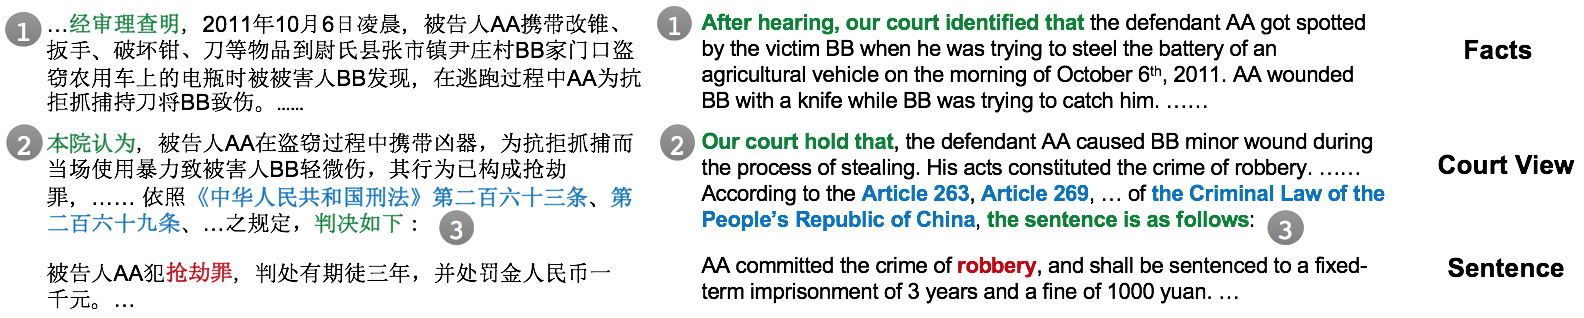
\includegraphics[width=0.97\textwidth]{figures/case.png}	
\caption{Example judgement document excerpt of a criminal case in China. Names are anonymized as AA and BB.
Rectangulars, ellipses and dashed rectangulars refer to the clauses that usually indicates the start of the facts part, the court view part and the sentence part, respectively.
}
\label{fig_example_case}
\end{center}
\end{figure*}
